% Created by tikzDevice version 0.12.3 on 2020-05-25 22:11:27
% !TEX encoding = UTF-8 Unicode
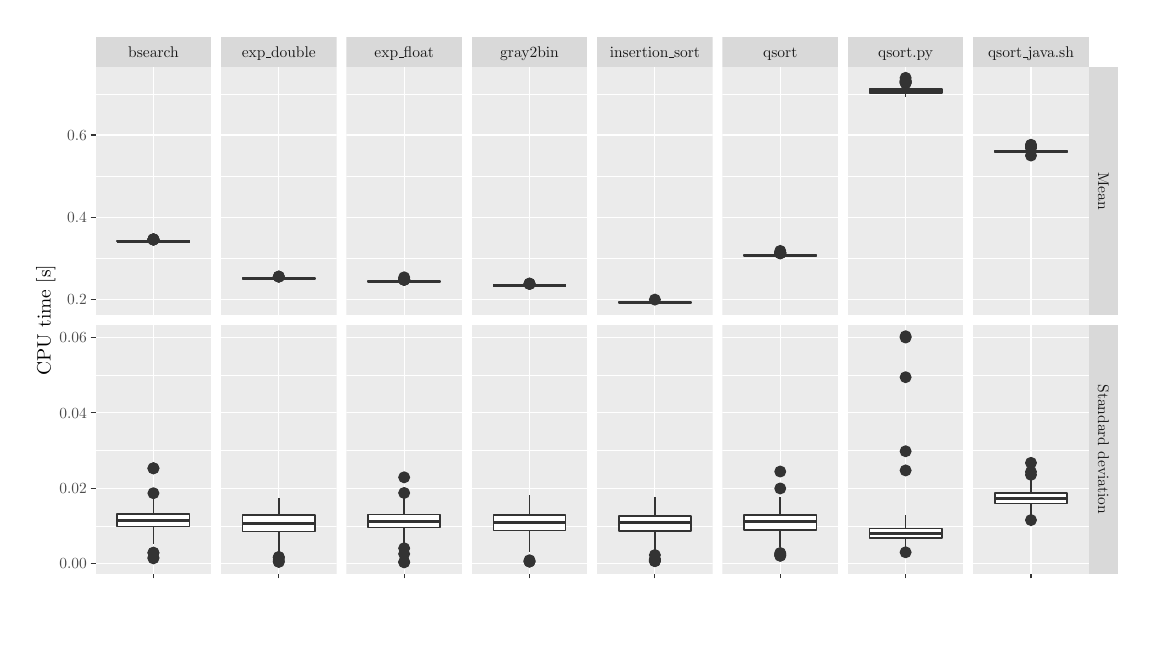
\begin{tikzpicture}[x=1pt,y=1pt]
\definecolor{fillColor}{RGB}{255,255,255}
\path[use as bounding box,fill=fillColor,fill opacity=0.00] (0,0) rectangle (397.48,216.81);
\begin{scope}
\path[clip] (  0.00,  0.00) rectangle (397.48,216.81);
\definecolor{drawColor}{RGB}{255,255,255}
\definecolor{fillColor}{RGB}{255,255,255}

\path[draw=drawColor,line width= 0.4pt,line join=round,line cap=round,fill=fillColor] ( -0.00,  0.00) rectangle (397.49,216.81);
\end{scope}
\begin{scope}
\path[clip] ( 24.53,112.90) rectangle ( 66.34,202.76);
\definecolor{fillColor}{gray}{0.92}

\path[fill=fillColor] ( 24.53,112.90) rectangle ( 66.34,202.76);
\definecolor{drawColor}{RGB}{255,255,255}

\path[draw=drawColor,line width= 0.2pt,line join=round] ( 24.53,133.45) --
	( 66.34,133.45);

\path[draw=drawColor,line width= 0.2pt,line join=round] ( 24.53,163.18) --
	( 66.34,163.18);

\path[draw=drawColor,line width= 0.2pt,line join=round] ( 24.53,192.91) --
	( 66.34,192.91);

\path[draw=drawColor,line width= 0.4pt,line join=round] ( 24.53,118.59) --
	( 66.34,118.59);

\path[draw=drawColor,line width= 0.4pt,line join=round] ( 24.53,148.32) --
	( 66.34,148.32);

\path[draw=drawColor,line width= 0.4pt,line join=round] ( 24.53,178.04) --
	( 66.34,178.04);

\path[draw=drawColor,line width= 0.4pt,line join=round] ( 45.44,112.90) --
	( 45.44,202.76);
\definecolor{drawColor}{gray}{0.20}
\definecolor{fillColor}{gray}{0.20}

\path[draw=drawColor,line width= 0.4pt,line join=round,line cap=round,fill=fillColor] ( 45.44,140.37) circle (  1.96);

\path[draw=drawColor,line width= 0.4pt,line join=round,line cap=round,fill=fillColor] ( 45.44,140.29) circle (  1.96);

\path[draw=drawColor,line width= 0.4pt,line join=round,line cap=round,fill=fillColor] ( 45.44,140.23) circle (  1.96);

\path[draw=drawColor,line width= 0.4pt,line join=round,line cap=round,fill=fillColor] ( 45.44,140.26) circle (  1.96);

\path[draw=drawColor,line width= 0.4pt,line join=round,line cap=round,fill=fillColor] ( 45.44,140.25) circle (  1.96);

\path[draw=drawColor,line width= 0.4pt,line join=round,line cap=round,fill=fillColor] ( 45.44,140.25) circle (  1.96);

\path[draw=drawColor,line width= 0.6pt,line join=round] ( 45.44,139.79) -- ( 45.44,140.21);

\path[draw=drawColor,line width= 0.6pt,line join=round] ( 45.44,139.51) -- ( 45.44,139.11);
\definecolor{fillColor}{RGB}{255,255,255}

\path[draw=drawColor,line width= 0.6pt,line join=round,line cap=round,fill=fillColor] ( 32.37,139.79) --
	( 32.37,139.51) --
	( 58.50,139.51) --
	( 58.50,139.79) --
	( 32.37,139.79) --
	cycle;

\path[draw=drawColor,line width= 1.1pt,line join=round] ( 32.37,139.64) -- ( 58.50,139.64);
\end{scope}
\begin{scope}
\path[clip] ( 24.53, 19.53) rectangle ( 66.34,109.40);
\definecolor{fillColor}{gray}{0.92}

\path[fill=fillColor] ( 24.53, 19.53) rectangle ( 66.34,109.40);
\definecolor{drawColor}{RGB}{255,255,255}

\path[draw=drawColor,line width= 0.2pt,line join=round] ( 24.53, 36.79) --
	( 66.34, 36.79);

\path[draw=drawColor,line width= 0.2pt,line join=round] ( 24.53, 64.01) --
	( 66.34, 64.01);

\path[draw=drawColor,line width= 0.2pt,line join=round] ( 24.53, 91.23) --
	( 66.34, 91.23);

\path[draw=drawColor,line width= 0.4pt,line join=round] ( 24.53, 23.19) --
	( 66.34, 23.19);

\path[draw=drawColor,line width= 0.4pt,line join=round] ( 24.53, 50.40) --
	( 66.34, 50.40);

\path[draw=drawColor,line width= 0.4pt,line join=round] ( 24.53, 77.62) --
	( 66.34, 77.62);

\path[draw=drawColor,line width= 0.4pt,line join=round] ( 24.53,104.84) --
	( 66.34,104.84);

\path[draw=drawColor,line width= 0.4pt,line join=round] ( 45.44, 19.53) --
	( 45.44,109.40);
\definecolor{drawColor}{gray}{0.20}
\definecolor{fillColor}{gray}{0.20}

\path[draw=drawColor,line width= 0.4pt,line join=round,line cap=round,fill=fillColor] ( 45.44, 27.10) circle (  1.96);

\path[draw=drawColor,line width= 0.4pt,line join=round,line cap=round,fill=fillColor] ( 45.44, 25.36) circle (  1.96);

\path[draw=drawColor,line width= 0.4pt,line join=round,line cap=round,fill=fillColor] ( 45.44, 57.63) circle (  1.96);

\path[draw=drawColor,line width= 0.4pt,line join=round,line cap=round,fill=fillColor] ( 45.44, 48.59) circle (  1.96);

\path[draw=drawColor,line width= 0.4pt,line join=round,line cap=round,fill=fillColor] ( 45.44, 57.56) circle (  1.96);

\path[draw=drawColor,line width= 0.4pt,line join=round,line cap=round,fill=fillColor] ( 45.44, 27.03) circle (  1.96);

\path[draw=drawColor,line width= 0.4pt,line join=round,line cap=round,fill=fillColor] ( 45.44, 25.05) circle (  1.96);

\path[draw=drawColor,line width= 0.6pt,line join=round] ( 45.44, 40.98) -- ( 45.44, 47.01);

\path[draw=drawColor,line width= 0.6pt,line join=round] ( 45.44, 36.60) -- ( 45.44, 30.06);
\definecolor{fillColor}{RGB}{255,255,255}

\path[draw=drawColor,line width= 0.6pt,line join=round,line cap=round,fill=fillColor] ( 32.37, 40.98) --
	( 32.37, 36.60) --
	( 58.50, 36.60) --
	( 58.50, 40.98) --
	( 32.37, 40.98) --
	cycle;

\path[draw=drawColor,line width= 1.1pt,line join=round] ( 32.37, 38.65) -- ( 58.50, 38.65);
\end{scope}
\begin{scope}
\path[clip] ( 69.84,112.90) rectangle (111.64,202.76);
\definecolor{fillColor}{gray}{0.92}

\path[fill=fillColor] ( 69.84,112.90) rectangle (111.64,202.76);
\definecolor{drawColor}{RGB}{255,255,255}

\path[draw=drawColor,line width= 0.2pt,line join=round] ( 69.84,133.45) --
	(111.64,133.45);

\path[draw=drawColor,line width= 0.2pt,line join=round] ( 69.84,163.18) --
	(111.64,163.18);

\path[draw=drawColor,line width= 0.2pt,line join=round] ( 69.84,192.91) --
	(111.64,192.91);

\path[draw=drawColor,line width= 0.4pt,line join=round] ( 69.84,118.59) --
	(111.64,118.59);

\path[draw=drawColor,line width= 0.4pt,line join=round] ( 69.84,148.32) --
	(111.64,148.32);

\path[draw=drawColor,line width= 0.4pt,line join=round] ( 69.84,178.04) --
	(111.64,178.04);

\path[draw=drawColor,line width= 0.4pt,line join=round] ( 90.74,112.90) --
	( 90.74,202.76);
\definecolor{drawColor}{gray}{0.20}
\definecolor{fillColor}{gray}{0.20}

\path[draw=drawColor,line width= 0.4pt,line join=round,line cap=round,fill=fillColor] ( 90.74,126.83) circle (  1.96);

\path[draw=drawColor,line width= 0.4pt,line join=round,line cap=round,fill=fillColor] ( 90.74,126.87) circle (  1.96);

\path[draw=drawColor,line width= 0.4pt,line join=round,line cap=round,fill=fillColor] ( 90.74,126.86) circle (  1.96);

\path[draw=drawColor,line width= 0.6pt,line join=round] ( 90.74,126.33) -- ( 90.74,126.77);

\path[draw=drawColor,line width= 0.6pt,line join=round] ( 90.74,126.03) -- ( 90.74,125.75);
\definecolor{fillColor}{RGB}{255,255,255}

\path[draw=drawColor,line width= 0.6pt,line join=round,line cap=round,fill=fillColor] ( 77.67,126.33) --
	( 77.67,126.03) --
	(103.80,126.03) --
	(103.80,126.33) --
	( 77.67,126.33) --
	cycle;

\path[draw=drawColor,line width= 1.1pt,line join=round] ( 77.67,126.18) -- (103.80,126.18);
\end{scope}
\begin{scope}
\path[clip] ( 69.84, 19.53) rectangle (111.64,109.40);
\definecolor{fillColor}{gray}{0.92}

\path[fill=fillColor] ( 69.84, 19.53) rectangle (111.64,109.40);
\definecolor{drawColor}{RGB}{255,255,255}

\path[draw=drawColor,line width= 0.2pt,line join=round] ( 69.84, 36.79) --
	(111.64, 36.79);

\path[draw=drawColor,line width= 0.2pt,line join=round] ( 69.84, 64.01) --
	(111.64, 64.01);

\path[draw=drawColor,line width= 0.2pt,line join=round] ( 69.84, 91.23) --
	(111.64, 91.23);

\path[draw=drawColor,line width= 0.4pt,line join=round] ( 69.84, 23.19) --
	(111.64, 23.19);

\path[draw=drawColor,line width= 0.4pt,line join=round] ( 69.84, 50.40) --
	(111.64, 50.40);

\path[draw=drawColor,line width= 0.4pt,line join=round] ( 69.84, 77.62) --
	(111.64, 77.62);

\path[draw=drawColor,line width= 0.4pt,line join=round] ( 69.84,104.84) --
	(111.64,104.84);

\path[draw=drawColor,line width= 0.4pt,line join=round] ( 90.74, 19.53) --
	( 90.74,109.40);
\definecolor{drawColor}{gray}{0.20}
\definecolor{fillColor}{gray}{0.20}

\path[draw=drawColor,line width= 0.4pt,line join=round,line cap=round,fill=fillColor] ( 90.74, 24.47) circle (  1.96);

\path[draw=drawColor,line width= 0.4pt,line join=round,line cap=round,fill=fillColor] ( 90.74, 25.40) circle (  1.96);

\path[draw=drawColor,line width= 0.4pt,line join=round,line cap=round,fill=fillColor] ( 90.74, 23.87) circle (  1.96);

\path[draw=drawColor,line width= 0.4pt,line join=round,line cap=round,fill=fillColor] ( 90.74, 25.56) circle (  1.96);

\path[draw=drawColor,line width= 0.4pt,line join=round,line cap=round,fill=fillColor] ( 90.74, 25.32) circle (  1.96);

\path[draw=drawColor,line width= 0.4pt,line join=round,line cap=round,fill=fillColor] ( 90.74, 23.77) circle (  1.96);

\path[draw=drawColor,line width= 0.6pt,line join=round] ( 90.74, 40.68) -- ( 90.74, 46.99);

\path[draw=drawColor,line width= 0.6pt,line join=round] ( 90.74, 34.80) -- ( 90.74, 26.16);
\definecolor{fillColor}{RGB}{255,255,255}

\path[draw=drawColor,line width= 0.6pt,line join=round,line cap=round,fill=fillColor] ( 77.67, 40.68) --
	( 77.67, 34.80) --
	(103.80, 34.80) --
	(103.80, 40.68) --
	( 77.67, 40.68) --
	cycle;

\path[draw=drawColor,line width= 1.1pt,line join=round] ( 77.67, 37.52) -- (103.80, 37.52);
\end{scope}
\begin{scope}
\path[clip] (115.14,112.90) rectangle (156.94,202.76);
\definecolor{fillColor}{gray}{0.92}

\path[fill=fillColor] (115.14,112.90) rectangle (156.94,202.76);
\definecolor{drawColor}{RGB}{255,255,255}

\path[draw=drawColor,line width= 0.2pt,line join=round] (115.14,133.45) --
	(156.94,133.45);

\path[draw=drawColor,line width= 0.2pt,line join=round] (115.14,163.18) --
	(156.94,163.18);

\path[draw=drawColor,line width= 0.2pt,line join=round] (115.14,192.91) --
	(156.94,192.91);

\path[draw=drawColor,line width= 0.4pt,line join=round] (115.14,118.59) --
	(156.94,118.59);

\path[draw=drawColor,line width= 0.4pt,line join=round] (115.14,148.32) --
	(156.94,148.32);

\path[draw=drawColor,line width= 0.4pt,line join=round] (115.14,178.04) --
	(156.94,178.04);

\path[draw=drawColor,line width= 0.4pt,line join=round] (136.04,112.90) --
	(136.04,202.76);
\definecolor{drawColor}{gray}{0.20}
\definecolor{fillColor}{gray}{0.20}

\path[draw=drawColor,line width= 0.4pt,line join=round,line cap=round,fill=fillColor] (136.04,126.60) circle (  1.96);

\path[draw=drawColor,line width= 0.4pt,line join=round,line cap=round,fill=fillColor] (136.04,125.78) circle (  1.96);

\path[draw=drawColor,line width= 0.4pt,line join=round,line cap=round,fill=fillColor] (136.04,125.70) circle (  1.96);

\path[draw=drawColor,line width= 0.4pt,line join=round,line cap=round,fill=fillColor] (136.04,125.68) circle (  1.96);

\path[draw=drawColor,line width= 0.4pt,line join=round,line cap=round,fill=fillColor] (136.04,125.71) circle (  1.96);

\path[draw=drawColor,line width= 0.4pt,line join=round,line cap=round,fill=fillColor] (136.04,125.88) circle (  1.96);

\path[draw=drawColor,line width= 0.6pt,line join=round] (136.04,125.24) -- (136.04,125.61);

\path[draw=drawColor,line width= 0.6pt,line join=round] (136.04,124.97) -- (136.04,124.60);
\definecolor{fillColor}{RGB}{255,255,255}

\path[draw=drawColor,line width= 0.6pt,line join=round,line cap=round,fill=fillColor] (122.97,125.24) --
	(122.97,124.97) --
	(149.10,124.97) --
	(149.10,125.24) --
	(122.97,125.24) --
	cycle;

\path[draw=drawColor,line width= 1.1pt,line join=round] (122.97,125.09) -- (149.10,125.09);
\end{scope}
\begin{scope}
\path[clip] (115.14, 19.53) rectangle (156.94,109.40);
\definecolor{fillColor}{gray}{0.92}

\path[fill=fillColor] (115.14, 19.53) rectangle (156.94,109.40);
\definecolor{drawColor}{RGB}{255,255,255}

\path[draw=drawColor,line width= 0.2pt,line join=round] (115.14, 36.79) --
	(156.94, 36.79);

\path[draw=drawColor,line width= 0.2pt,line join=round] (115.14, 64.01) --
	(156.94, 64.01);

\path[draw=drawColor,line width= 0.2pt,line join=round] (115.14, 91.23) --
	(156.94, 91.23);

\path[draw=drawColor,line width= 0.4pt,line join=round] (115.14, 23.19) --
	(156.94, 23.19);

\path[draw=drawColor,line width= 0.4pt,line join=round] (115.14, 50.40) --
	(156.94, 50.40);

\path[draw=drawColor,line width= 0.4pt,line join=round] (115.14, 77.62) --
	(156.94, 77.62);

\path[draw=drawColor,line width= 0.4pt,line join=round] (115.14,104.84) --
	(156.94,104.84);

\path[draw=drawColor,line width= 0.4pt,line join=round] (136.04, 19.53) --
	(136.04,109.40);
\definecolor{drawColor}{gray}{0.20}
\definecolor{fillColor}{gray}{0.20}

\path[draw=drawColor,line width= 0.4pt,line join=round,line cap=round,fill=fillColor] (136.04, 54.33) circle (  1.96);

\path[draw=drawColor,line width= 0.4pt,line join=round,line cap=round,fill=fillColor] (136.04, 23.61) circle (  1.96);

\path[draw=drawColor,line width= 0.4pt,line join=round,line cap=round,fill=fillColor] (136.04, 26.65) circle (  1.96);

\path[draw=drawColor,line width= 0.4pt,line join=round,line cap=round,fill=fillColor] (136.04, 23.75) circle (  1.96);

\path[draw=drawColor,line width= 0.4pt,line join=round,line cap=round,fill=fillColor] (136.04, 28.70) circle (  1.96);

\path[draw=drawColor,line width= 0.4pt,line join=round,line cap=round,fill=fillColor] (136.04, 48.68) circle (  1.96);

\path[draw=drawColor,line width= 0.6pt,line join=round] (136.04, 40.90) -- (136.04, 47.23);

\path[draw=drawColor,line width= 0.6pt,line join=round] (136.04, 36.18) -- (136.04, 29.19);
\definecolor{fillColor}{RGB}{255,255,255}

\path[draw=drawColor,line width= 0.6pt,line join=round,line cap=round,fill=fillColor] (122.97, 40.90) --
	(122.97, 36.18) --
	(149.10, 36.18) --
	(149.10, 40.90) --
	(122.97, 40.90) --
	cycle;

\path[draw=drawColor,line width= 1.1pt,line join=round] (122.97, 38.42) -- (149.10, 38.42);
\end{scope}
\begin{scope}
\path[clip] (160.44,112.90) rectangle (202.24,202.76);
\definecolor{fillColor}{gray}{0.92}

\path[fill=fillColor] (160.44,112.90) rectangle (202.24,202.76);
\definecolor{drawColor}{RGB}{255,255,255}

\path[draw=drawColor,line width= 0.2pt,line join=round] (160.44,133.45) --
	(202.24,133.45);

\path[draw=drawColor,line width= 0.2pt,line join=round] (160.44,163.18) --
	(202.24,163.18);

\path[draw=drawColor,line width= 0.2pt,line join=round] (160.44,192.91) --
	(202.24,192.91);

\path[draw=drawColor,line width= 0.4pt,line join=round] (160.44,118.59) --
	(202.24,118.59);

\path[draw=drawColor,line width= 0.4pt,line join=round] (160.44,148.32) --
	(202.24,148.32);

\path[draw=drawColor,line width= 0.4pt,line join=round] (160.44,178.04) --
	(202.24,178.04);

\path[draw=drawColor,line width= 0.4pt,line join=round] (181.34,112.90) --
	(181.34,202.76);
\definecolor{drawColor}{gray}{0.20}
\definecolor{fillColor}{gray}{0.20}

\path[draw=drawColor,line width= 0.4pt,line join=round,line cap=round,fill=fillColor] (181.34,124.23) circle (  1.96);

\path[draw=drawColor,line width= 0.4pt,line join=round,line cap=round,fill=fillColor] (181.34,124.30) circle (  1.96);

\path[draw=drawColor,line width= 0.4pt,line join=round,line cap=round,fill=fillColor] (181.34,124.20) circle (  1.96);

\path[draw=drawColor,line width= 0.4pt,line join=round,line cap=round,fill=fillColor] (181.34,124.35) circle (  1.96);

\path[draw=drawColor,line width= 0.6pt,line join=round] (181.34,123.74) -- (181.34,124.19);

\path[draw=drawColor,line width= 0.6pt,line join=round] (181.34,123.44) -- (181.34,123.08);
\definecolor{fillColor}{RGB}{255,255,255}

\path[draw=drawColor,line width= 0.6pt,line join=round,line cap=round,fill=fillColor] (168.27,123.74) --
	(168.27,123.44) --
	(194.40,123.44) --
	(194.40,123.74) --
	(168.27,123.74) --
	cycle;

\path[draw=drawColor,line width= 1.1pt,line join=round] (168.27,123.60) -- (194.40,123.60);
\end{scope}
\begin{scope}
\path[clip] (160.44, 19.53) rectangle (202.24,109.40);
\definecolor{fillColor}{gray}{0.92}

\path[fill=fillColor] (160.44, 19.53) rectangle (202.24,109.40);
\definecolor{drawColor}{RGB}{255,255,255}

\path[draw=drawColor,line width= 0.2pt,line join=round] (160.44, 36.79) --
	(202.24, 36.79);

\path[draw=drawColor,line width= 0.2pt,line join=round] (160.44, 64.01) --
	(202.24, 64.01);

\path[draw=drawColor,line width= 0.2pt,line join=round] (160.44, 91.23) --
	(202.24, 91.23);

\path[draw=drawColor,line width= 0.4pt,line join=round] (160.44, 23.19) --
	(202.24, 23.19);

\path[draw=drawColor,line width= 0.4pt,line join=round] (160.44, 50.40) --
	(202.24, 50.40);

\path[draw=drawColor,line width= 0.4pt,line join=round] (160.44, 77.62) --
	(202.24, 77.62);

\path[draw=drawColor,line width= 0.4pt,line join=round] (160.44,104.84) --
	(202.24,104.84);

\path[draw=drawColor,line width= 0.4pt,line join=round] (181.34, 19.53) --
	(181.34,109.40);
\definecolor{drawColor}{gray}{0.20}
\definecolor{fillColor}{gray}{0.20}

\path[draw=drawColor,line width= 0.4pt,line join=round,line cap=round,fill=fillColor] (181.34, 24.37) circle (  1.96);

\path[draw=drawColor,line width= 0.4pt,line join=round,line cap=round,fill=fillColor] (181.34, 23.91) circle (  1.96);

\path[draw=drawColor,line width= 0.4pt,line join=round,line cap=round,fill=fillColor] (181.34, 23.88) circle (  1.96);

\path[draw=drawColor,line width= 0.4pt,line join=round,line cap=round,fill=fillColor] (181.34, 23.92) circle (  1.96);

\path[draw=drawColor,line width= 0.6pt,line join=round] (181.34, 40.63) -- (181.34, 47.84);

\path[draw=drawColor,line width= 0.6pt,line join=round] (181.34, 35.08) -- (181.34, 27.51);
\definecolor{fillColor}{RGB}{255,255,255}

\path[draw=drawColor,line width= 0.6pt,line join=round,line cap=round,fill=fillColor] (168.27, 40.63) --
	(168.27, 35.08) --
	(194.40, 35.08) --
	(194.40, 40.63) --
	(168.27, 40.63) --
	cycle;

\path[draw=drawColor,line width= 1.1pt,line join=round] (168.27, 37.91) -- (194.40, 37.91);
\end{scope}
\begin{scope}
\path[clip] (205.74,112.90) rectangle (247.54,202.76);
\definecolor{fillColor}{gray}{0.92}

\path[fill=fillColor] (205.74,112.90) rectangle (247.54,202.76);
\definecolor{drawColor}{RGB}{255,255,255}

\path[draw=drawColor,line width= 0.2pt,line join=round] (205.74,133.45) --
	(247.54,133.45);

\path[draw=drawColor,line width= 0.2pt,line join=round] (205.74,163.18) --
	(247.54,163.18);

\path[draw=drawColor,line width= 0.2pt,line join=round] (205.74,192.91) --
	(247.54,192.91);

\path[draw=drawColor,line width= 0.4pt,line join=round] (205.74,118.59) --
	(247.54,118.59);

\path[draw=drawColor,line width= 0.4pt,line join=round] (205.74,148.32) --
	(247.54,148.32);

\path[draw=drawColor,line width= 0.4pt,line join=round] (205.74,178.04) --
	(247.54,178.04);

\path[draw=drawColor,line width= 0.4pt,line join=round] (226.64,112.90) --
	(226.64,202.76);
\definecolor{drawColor}{gray}{0.20}
\definecolor{fillColor}{gray}{0.20}

\path[draw=drawColor,line width= 0.4pt,line join=round,line cap=round,fill=fillColor] (226.64,118.54) circle (  1.96);

\path[draw=drawColor,line width= 0.6pt,line join=round] (226.64,117.70) -- (226.64,118.16);

\path[draw=drawColor,line width= 0.6pt,line join=round] (226.64,117.38) -- (226.64,116.98);
\definecolor{fillColor}{RGB}{255,255,255}

\path[draw=drawColor,line width= 0.6pt,line join=round,line cap=round,fill=fillColor] (213.57,117.70) --
	(213.57,117.38) --
	(239.70,117.38) --
	(239.70,117.70) --
	(213.57,117.70) --
	cycle;

\path[draw=drawColor,line width= 1.1pt,line join=round] (213.57,117.54) -- (239.70,117.54);
\end{scope}
\begin{scope}
\path[clip] (205.74, 19.53) rectangle (247.54,109.40);
\definecolor{fillColor}{gray}{0.92}

\path[fill=fillColor] (205.74, 19.53) rectangle (247.54,109.40);
\definecolor{drawColor}{RGB}{255,255,255}

\path[draw=drawColor,line width= 0.2pt,line join=round] (205.74, 36.79) --
	(247.54, 36.79);

\path[draw=drawColor,line width= 0.2pt,line join=round] (205.74, 64.01) --
	(247.54, 64.01);

\path[draw=drawColor,line width= 0.2pt,line join=round] (205.74, 91.23) --
	(247.54, 91.23);

\path[draw=drawColor,line width= 0.4pt,line join=round] (205.74, 23.19) --
	(247.54, 23.19);

\path[draw=drawColor,line width= 0.4pt,line join=round] (205.74, 50.40) --
	(247.54, 50.40);

\path[draw=drawColor,line width= 0.4pt,line join=round] (205.74, 77.62) --
	(247.54, 77.62);

\path[draw=drawColor,line width= 0.4pt,line join=round] (205.74,104.84) --
	(247.54,104.84);

\path[draw=drawColor,line width= 0.4pt,line join=round] (226.64, 19.53) --
	(226.64,109.40);
\definecolor{drawColor}{gray}{0.20}
\definecolor{fillColor}{gray}{0.20}

\path[draw=drawColor,line width= 0.4pt,line join=round,line cap=round,fill=fillColor] (226.64, 26.24) circle (  1.96);

\path[draw=drawColor,line width= 0.4pt,line join=round,line cap=round,fill=fillColor] (226.64, 24.72) circle (  1.96);

\path[draw=drawColor,line width= 0.4pt,line join=round,line cap=round,fill=fillColor] (226.64, 24.77) circle (  1.96);

\path[draw=drawColor,line width= 0.4pt,line join=round,line cap=round,fill=fillColor] (226.64, 24.21) circle (  1.96);

\path[draw=drawColor,line width= 0.4pt,line join=round,line cap=round,fill=fillColor] (226.64, 24.12) circle (  1.96);

\path[draw=drawColor,line width= 0.4pt,line join=round,line cap=round,fill=fillColor] (226.64, 24.01) circle (  1.96);

\path[draw=drawColor,line width= 0.6pt,line join=round] (226.64, 40.26) -- (226.64, 47.36);

\path[draw=drawColor,line width= 0.6pt,line join=round] (226.64, 35.00) -- (226.64, 28.22);
\definecolor{fillColor}{RGB}{255,255,255}

\path[draw=drawColor,line width= 0.6pt,line join=round,line cap=round,fill=fillColor] (213.57, 40.26) --
	(213.57, 35.00) --
	(239.70, 35.00) --
	(239.70, 40.26) --
	(213.57, 40.26) --
	cycle;

\path[draw=drawColor,line width= 1.1pt,line join=round] (213.57, 37.99) -- (239.70, 37.99);
\end{scope}
\begin{scope}
\path[clip] (251.04,112.90) rectangle (292.84,202.76);
\definecolor{fillColor}{gray}{0.92}

\path[fill=fillColor] (251.04,112.90) rectangle (292.84,202.76);
\definecolor{drawColor}{RGB}{255,255,255}

\path[draw=drawColor,line width= 0.2pt,line join=round] (251.04,133.45) --
	(292.84,133.45);

\path[draw=drawColor,line width= 0.2pt,line join=round] (251.04,163.18) --
	(292.84,163.18);

\path[draw=drawColor,line width= 0.2pt,line join=round] (251.04,192.91) --
	(292.84,192.91);

\path[draw=drawColor,line width= 0.4pt,line join=round] (251.04,118.59) --
	(292.84,118.59);

\path[draw=drawColor,line width= 0.4pt,line join=round] (251.04,148.32) --
	(292.84,148.32);

\path[draw=drawColor,line width= 0.4pt,line join=round] (251.04,178.04) --
	(292.84,178.04);

\path[draw=drawColor,line width= 0.4pt,line join=round] (271.94,112.90) --
	(271.94,202.76);
\definecolor{drawColor}{gray}{0.20}
\definecolor{fillColor}{gray}{0.20}

\path[draw=drawColor,line width= 0.4pt,line join=round,line cap=round,fill=fillColor] (271.94,135.28) circle (  1.96);

\path[draw=drawColor,line width= 0.4pt,line join=round,line cap=round,fill=fillColor] (271.94,136.14) circle (  1.96);

\path[draw=drawColor,line width= 0.4pt,line join=round,line cap=round,fill=fillColor] (271.94,135.40) circle (  1.96);

\path[draw=drawColor,line width= 0.4pt,line join=round,line cap=round,fill=fillColor] (271.94,135.48) circle (  1.96);

\path[draw=drawColor,line width= 0.4pt,line join=round,line cap=round,fill=fillColor] (271.94,135.42) circle (  1.96);

\path[draw=drawColor,line width= 0.4pt,line join=round,line cap=round,fill=fillColor] (271.94,135.41) circle (  1.96);

\path[draw=drawColor,line width= 0.4pt,line join=round,line cap=round,fill=fillColor] (271.94,135.26) circle (  1.96);

\path[draw=drawColor,line width= 0.4pt,line join=round,line cap=round,fill=fillColor] (271.94,135.43) circle (  1.96);

\path[draw=drawColor,line width= 0.4pt,line join=round,line cap=round,fill=fillColor] (271.94,135.50) circle (  1.96);

\path[draw=drawColor,line width= 0.6pt,line join=round] (271.94,134.65) -- (271.94,135.18);

\path[draw=drawColor,line width= 0.6pt,line join=round] (271.94,134.27) -- (271.94,133.87);
\definecolor{fillColor}{RGB}{255,255,255}

\path[draw=drawColor,line width= 0.6pt,line join=round,line cap=round,fill=fillColor] (258.88,134.65) --
	(258.88,134.27) --
	(285.00,134.27) --
	(285.00,134.65) --
	(258.88,134.65) --
	cycle;

\path[draw=drawColor,line width= 1.1pt,line join=round] (258.88,134.47) -- (285.00,134.47);
\end{scope}
\begin{scope}
\path[clip] (251.04, 19.53) rectangle (292.84,109.40);
\definecolor{fillColor}{gray}{0.92}

\path[fill=fillColor] (251.04, 19.53) rectangle (292.84,109.40);
\definecolor{drawColor}{RGB}{255,255,255}

\path[draw=drawColor,line width= 0.2pt,line join=round] (251.04, 36.79) --
	(292.84, 36.79);

\path[draw=drawColor,line width= 0.2pt,line join=round] (251.04, 64.01) --
	(292.84, 64.01);

\path[draw=drawColor,line width= 0.2pt,line join=round] (251.04, 91.23) --
	(292.84, 91.23);

\path[draw=drawColor,line width= 0.4pt,line join=round] (251.04, 23.19) --
	(292.84, 23.19);

\path[draw=drawColor,line width= 0.4pt,line join=round] (251.04, 50.40) --
	(292.84, 50.40);

\path[draw=drawColor,line width= 0.4pt,line join=round] (251.04, 77.62) --
	(292.84, 77.62);

\path[draw=drawColor,line width= 0.4pt,line join=round] (251.04,104.84) --
	(292.84,104.84);

\path[draw=drawColor,line width= 0.4pt,line join=round] (271.94, 19.53) --
	(271.94,109.40);
\definecolor{drawColor}{gray}{0.20}
\definecolor{fillColor}{gray}{0.20}

\path[draw=drawColor,line width= 0.4pt,line join=round,line cap=round,fill=fillColor] (271.94, 50.31) circle (  1.96);

\path[draw=drawColor,line width= 0.4pt,line join=round,line cap=round,fill=fillColor] (271.94, 26.68) circle (  1.96);

\path[draw=drawColor,line width= 0.4pt,line join=round,line cap=round,fill=fillColor] (271.94, 26.04) circle (  1.96);

\path[draw=drawColor,line width= 0.4pt,line join=round,line cap=round,fill=fillColor] (271.94, 25.97) circle (  1.96);

\path[draw=drawColor,line width= 0.4pt,line join=round,line cap=round,fill=fillColor] (271.94, 26.32) circle (  1.96);

\path[draw=drawColor,line width= 0.4pt,line join=round,line cap=round,fill=fillColor] (271.94, 56.42) circle (  1.96);

\path[draw=drawColor,line width= 0.4pt,line join=round,line cap=round,fill=fillColor] (271.94, 26.98) circle (  1.96);

\path[draw=drawColor,line width= 0.6pt,line join=round] (271.94, 40.72) -- (271.94, 47.36);

\path[draw=drawColor,line width= 0.6pt,line join=round] (271.94, 35.27) -- (271.94, 29.04);
\definecolor{fillColor}{RGB}{255,255,255}

\path[draw=drawColor,line width= 0.6pt,line join=round,line cap=round,fill=fillColor] (258.88, 40.72) --
	(258.88, 35.27) --
	(285.00, 35.27) --
	(285.00, 40.72) --
	(258.88, 40.72) --
	cycle;

\path[draw=drawColor,line width= 1.1pt,line join=round] (258.88, 38.30) -- (285.00, 38.30);
\end{scope}
\begin{scope}
\path[clip] (296.34,112.90) rectangle (338.14,202.76);
\definecolor{fillColor}{gray}{0.92}

\path[fill=fillColor] (296.34,112.90) rectangle (338.14,202.76);
\definecolor{drawColor}{RGB}{255,255,255}

\path[draw=drawColor,line width= 0.2pt,line join=round] (296.34,133.45) --
	(338.14,133.45);

\path[draw=drawColor,line width= 0.2pt,line join=round] (296.34,163.18) --
	(338.14,163.18);

\path[draw=drawColor,line width= 0.2pt,line join=round] (296.34,192.91) --
	(338.14,192.91);

\path[draw=drawColor,line width= 0.4pt,line join=round] (296.34,118.59) --
	(338.14,118.59);

\path[draw=drawColor,line width= 0.4pt,line join=round] (296.34,148.32) --
	(338.14,148.32);

\path[draw=drawColor,line width= 0.4pt,line join=round] (296.34,178.04) --
	(338.14,178.04);

\path[draw=drawColor,line width= 0.4pt,line join=round] (317.24,112.90) --
	(317.24,202.76);
\definecolor{drawColor}{gray}{0.20}
\definecolor{fillColor}{gray}{0.20}

\path[draw=drawColor,line width= 0.4pt,line join=round,line cap=round,fill=fillColor] (317.24,197.77) circle (  1.96);

\path[draw=drawColor,line width= 0.4pt,line join=round,line cap=round,fill=fillColor] (317.24,198.68) circle (  1.96);

\path[draw=drawColor,line width= 0.4pt,line join=round,line cap=round,fill=fillColor] (317.24,197.33) circle (  1.96);

\path[draw=drawColor,line width= 0.4pt,line join=round,line cap=round,fill=fillColor] (317.24,196.78) circle (  1.96);

\path[draw=drawColor,line width= 0.4pt,line join=round,line cap=round,fill=fillColor] (317.24,197.47) circle (  1.96);

\path[draw=drawColor,line width= 0.4pt,line join=round,line cap=round,fill=fillColor] (317.24,196.80) circle (  1.96);

\path[draw=drawColor,line width= 0.4pt,line join=round,line cap=round,fill=fillColor] (317.24,197.05) circle (  1.96);

\path[draw=drawColor,line width= 0.6pt,line join=round] (317.24,194.62) -- (317.24,196.55);

\path[draw=drawColor,line width= 0.6pt,line join=round] (317.24,193.29) -- (317.24,191.81);
\definecolor{fillColor}{RGB}{255,255,255}

\path[draw=drawColor,line width= 0.6pt,line join=round,line cap=round,fill=fillColor] (304.18,194.62) --
	(304.18,193.29) --
	(330.30,193.29) --
	(330.30,194.62) --
	(304.18,194.62) --
	cycle;

\path[draw=drawColor,line width= 1.1pt,line join=round] (304.18,193.92) -- (330.30,193.92);
\end{scope}
\begin{scope}
\path[clip] (296.34, 19.53) rectangle (338.14,109.40);
\definecolor{fillColor}{gray}{0.92}

\path[fill=fillColor] (296.34, 19.53) rectangle (338.14,109.40);
\definecolor{drawColor}{RGB}{255,255,255}

\path[draw=drawColor,line width= 0.2pt,line join=round] (296.34, 36.79) --
	(338.14, 36.79);

\path[draw=drawColor,line width= 0.2pt,line join=round] (296.34, 64.01) --
	(338.14, 64.01);

\path[draw=drawColor,line width= 0.2pt,line join=round] (296.34, 91.23) --
	(338.14, 91.23);

\path[draw=drawColor,line width= 0.4pt,line join=round] (296.34, 23.19) --
	(338.14, 23.19);

\path[draw=drawColor,line width= 0.4pt,line join=round] (296.34, 50.40) --
	(338.14, 50.40);

\path[draw=drawColor,line width= 0.4pt,line join=round] (296.34, 77.62) --
	(338.14, 77.62);

\path[draw=drawColor,line width= 0.4pt,line join=round] (296.34,104.84) --
	(338.14,104.84);

\path[draw=drawColor,line width= 0.4pt,line join=round] (317.24, 19.53) --
	(317.24,109.40);
\definecolor{drawColor}{gray}{0.20}
\definecolor{fillColor}{gray}{0.20}

\path[draw=drawColor,line width= 0.4pt,line join=round,line cap=round,fill=fillColor] (317.24, 56.82) circle (  1.96);

\path[draw=drawColor,line width= 0.4pt,line join=round,line cap=round,fill=fillColor] (317.24,104.84) circle (  1.96);

\path[draw=drawColor,line width= 0.4pt,line join=round,line cap=round,fill=fillColor] (317.24, 90.51) circle (  1.96);

\path[draw=drawColor,line width= 0.4pt,line join=round,line cap=round,fill=fillColor] (317.24, 63.75) circle (  1.96);

\path[draw=drawColor,line width= 0.4pt,line join=round,line cap=round,fill=fillColor] (317.24,105.31) circle (  1.96);

\path[draw=drawColor,line width= 0.4pt,line join=round,line cap=round,fill=fillColor] (317.24, 27.24) circle (  1.96);

\path[draw=drawColor,line width= 0.6pt,line join=round] (317.24, 35.82) -- (317.24, 40.86);

\path[draw=drawColor,line width= 0.6pt,line join=round] (317.24, 32.45) -- (317.24, 28.82);
\definecolor{fillColor}{RGB}{255,255,255}

\path[draw=drawColor,line width= 0.6pt,line join=round,line cap=round,fill=fillColor] (304.18, 35.82) --
	(304.18, 32.45) --
	(330.30, 32.45) --
	(330.30, 35.82) --
	(304.18, 35.82) --
	cycle;

\path[draw=drawColor,line width= 1.1pt,line join=round] (304.18, 34.12) -- (330.30, 34.12);
\end{scope}
\begin{scope}
\path[clip] (341.64,112.90) rectangle (383.44,202.76);
\definecolor{fillColor}{gray}{0.92}

\path[fill=fillColor] (341.64,112.90) rectangle (383.44,202.76);
\definecolor{drawColor}{RGB}{255,255,255}

\path[draw=drawColor,line width= 0.2pt,line join=round] (341.64,133.45) --
	(383.44,133.45);

\path[draw=drawColor,line width= 0.2pt,line join=round] (341.64,163.18) --
	(383.44,163.18);

\path[draw=drawColor,line width= 0.2pt,line join=round] (341.64,192.91) --
	(383.44,192.91);

\path[draw=drawColor,line width= 0.4pt,line join=round] (341.64,118.59) --
	(383.44,118.59);

\path[draw=drawColor,line width= 0.4pt,line join=round] (341.64,148.32) --
	(383.44,148.32);

\path[draw=drawColor,line width= 0.4pt,line join=round] (341.64,178.04) --
	(383.44,178.04);

\path[draw=drawColor,line width= 0.4pt,line join=round] (362.54,112.90) --
	(362.54,202.76);
\definecolor{drawColor}{gray}{0.20}
\definecolor{fillColor}{gray}{0.20}

\path[draw=drawColor,line width= 0.4pt,line join=round,line cap=round,fill=fillColor] (362.54,174.50) circle (  1.96);

\path[draw=drawColor,line width= 0.4pt,line join=round,line cap=round,fill=fillColor] (362.54,170.60) circle (  1.96);

\path[draw=drawColor,line width= 0.4pt,line join=round,line cap=round,fill=fillColor] (362.54,174.14) circle (  1.96);

\path[draw=drawColor,line width= 0.4pt,line join=round,line cap=round,fill=fillColor] (362.54,173.70) circle (  1.96);

\path[draw=drawColor,line width= 0.4pt,line join=round,line cap=round,fill=fillColor] (362.54,173.64) circle (  1.96);

\path[draw=drawColor,line width= 0.4pt,line join=round,line cap=round,fill=fillColor] (362.54,173.58) circle (  1.96);

\path[draw=drawColor,line width= 0.4pt,line join=round,line cap=round,fill=fillColor] (362.54,174.02) circle (  1.96);

\path[draw=drawColor,line width= 0.4pt,line join=round,line cap=round,fill=fillColor] (362.54,173.55) circle (  1.96);

\path[draw=drawColor,line width= 0.4pt,line join=round,line cap=round,fill=fillColor] (362.54,173.65) circle (  1.96);

\path[draw=drawColor,line width= 0.4pt,line join=round,line cap=round,fill=fillColor] (362.54,173.92) circle (  1.96);

\path[draw=drawColor,line width= 0.4pt,line join=round,line cap=round,fill=fillColor] (362.54,174.17) circle (  1.96);

\path[draw=drawColor,line width= 0.4pt,line join=round,line cap=round,fill=fillColor] (362.54,173.62) circle (  1.96);

\path[draw=drawColor,line width= 0.6pt,line join=round] (362.54,172.46) -- (362.54,173.52);

\path[draw=drawColor,line width= 0.6pt,line join=round] (362.54,171.75) -- (362.54,170.87);
\definecolor{fillColor}{RGB}{255,255,255}

\path[draw=drawColor,line width= 0.6pt,line join=round,line cap=round,fill=fillColor] (349.48,172.46) --
	(349.48,171.75) --
	(375.60,171.75) --
	(375.60,172.46) --
	(349.48,172.46) --
	cycle;

\path[draw=drawColor,line width= 1.1pt,line join=round] (349.48,172.10) -- (375.60,172.10);
\end{scope}
\begin{scope}
\path[clip] (341.64, 19.53) rectangle (383.44,109.40);
\definecolor{fillColor}{gray}{0.92}

\path[fill=fillColor] (341.64, 19.53) rectangle (383.44,109.40);
\definecolor{drawColor}{RGB}{255,255,255}

\path[draw=drawColor,line width= 0.2pt,line join=round] (341.64, 36.79) --
	(383.44, 36.79);

\path[draw=drawColor,line width= 0.2pt,line join=round] (341.64, 64.01) --
	(383.44, 64.01);

\path[draw=drawColor,line width= 0.2pt,line join=round] (341.64, 91.23) --
	(383.44, 91.23);

\path[draw=drawColor,line width= 0.4pt,line join=round] (341.64, 23.19) --
	(383.44, 23.19);

\path[draw=drawColor,line width= 0.4pt,line join=round] (341.64, 50.40) --
	(383.44, 50.40);

\path[draw=drawColor,line width= 0.4pt,line join=round] (341.64, 77.62) --
	(383.44, 77.62);

\path[draw=drawColor,line width= 0.4pt,line join=round] (341.64,104.84) --
	(383.44,104.84);

\path[draw=drawColor,line width= 0.4pt,line join=round] (362.54, 19.53) --
	(362.54,109.40);
\definecolor{drawColor}{gray}{0.20}
\definecolor{fillColor}{gray}{0.20}

\path[draw=drawColor,line width= 0.4pt,line join=round,line cap=round,fill=fillColor] (362.54, 38.88) circle (  1.96);

\path[draw=drawColor,line width= 0.4pt,line join=round,line cap=round,fill=fillColor] (362.54, 55.24) circle (  1.96);

\path[draw=drawColor,line width= 0.4pt,line join=round,line cap=round,fill=fillColor] (362.54, 56.31) circle (  1.96);

\path[draw=drawColor,line width= 0.4pt,line join=round,line cap=round,fill=fillColor] (362.54, 59.56) circle (  1.96);

\path[draw=drawColor,line width= 0.6pt,line join=round] (362.54, 48.70) -- (362.54, 53.76);

\path[draw=drawColor,line width= 0.6pt,line join=round] (362.54, 44.81) -- (362.54, 39.82);
\definecolor{fillColor}{RGB}{255,255,255}

\path[draw=drawColor,line width= 0.6pt,line join=round,line cap=round,fill=fillColor] (349.48, 48.70) --
	(349.48, 44.81) --
	(375.60, 44.81) --
	(375.60, 48.70) --
	(349.48, 48.70) --
	cycle;

\path[draw=drawColor,line width= 1.1pt,line join=round] (349.48, 46.66) -- (375.60, 46.66);
\end{scope}
\begin{scope}
\path[clip] ( 24.53,202.76) rectangle ( 66.34,213.31);
\definecolor{fillColor}{gray}{0.85}

\path[fill=fillColor] ( 24.53,202.76) rectangle ( 66.34,213.31);
\definecolor{drawColor}{gray}{0.10}

\node[text=drawColor,anchor=base,inner sep=0pt, outer sep=0pt, scale=  0.56] at ( 45.44,206.11) {bsearch};
\end{scope}
\begin{scope}
\path[clip] ( 69.84,202.76) rectangle (111.64,213.31);
\definecolor{fillColor}{gray}{0.85}

\path[fill=fillColor] ( 69.84,202.76) rectangle (111.64,213.31);
\definecolor{drawColor}{gray}{0.10}

\node[text=drawColor,anchor=base,inner sep=0pt, outer sep=0pt, scale=  0.56] at ( 90.74,206.11) {exp\_double};
\end{scope}
\begin{scope}
\path[clip] (115.14,202.76) rectangle (156.94,213.31);
\definecolor{fillColor}{gray}{0.85}

\path[fill=fillColor] (115.14,202.76) rectangle (156.94,213.31);
\definecolor{drawColor}{gray}{0.10}

\node[text=drawColor,anchor=base,inner sep=0pt, outer sep=0pt, scale=  0.56] at (136.04,206.11) {exp\_float};
\end{scope}
\begin{scope}
\path[clip] (160.44,202.76) rectangle (202.24,213.31);
\definecolor{fillColor}{gray}{0.85}

\path[fill=fillColor] (160.44,202.76) rectangle (202.24,213.31);
\definecolor{drawColor}{gray}{0.10}

\node[text=drawColor,anchor=base,inner sep=0pt, outer sep=0pt, scale=  0.56] at (181.34,206.11) {gray2bin};
\end{scope}
\begin{scope}
\path[clip] (205.74,202.76) rectangle (247.54,213.31);
\definecolor{fillColor}{gray}{0.85}

\path[fill=fillColor] (205.74,202.76) rectangle (247.54,213.31);
\definecolor{drawColor}{gray}{0.10}

\node[text=drawColor,anchor=base,inner sep=0pt, outer sep=0pt, scale=  0.56] at (226.64,206.11) {insertion\_sort};
\end{scope}
\begin{scope}
\path[clip] (251.04,202.76) rectangle (292.84,213.31);
\definecolor{fillColor}{gray}{0.85}

\path[fill=fillColor] (251.04,202.76) rectangle (292.84,213.31);
\definecolor{drawColor}{gray}{0.10}

\node[text=drawColor,anchor=base,inner sep=0pt, outer sep=0pt, scale=  0.56] at (271.94,206.11) {qsort};
\end{scope}
\begin{scope}
\path[clip] (296.34,202.76) rectangle (338.14,213.31);
\definecolor{fillColor}{gray}{0.85}

\path[fill=fillColor] (296.34,202.76) rectangle (338.14,213.31);
\definecolor{drawColor}{gray}{0.10}

\node[text=drawColor,anchor=base,inner sep=0pt, outer sep=0pt, scale=  0.56] at (317.24,206.11) {qsort.py};
\end{scope}
\begin{scope}
\path[clip] (341.64,202.76) rectangle (383.44,213.31);
\definecolor{fillColor}{gray}{0.85}

\path[fill=fillColor] (341.64,202.76) rectangle (383.44,213.31);
\definecolor{drawColor}{gray}{0.10}

\node[text=drawColor,anchor=base,inner sep=0pt, outer sep=0pt, scale=  0.56] at (362.54,206.11) {qsort\_java.sh};
\end{scope}
\begin{scope}
\path[clip] (383.44,112.90) rectangle (393.98,202.76);
\definecolor{fillColor}{gray}{0.85}

\path[fill=fillColor] (383.44,112.90) rectangle (393.98,202.76);
\definecolor{drawColor}{gray}{0.10}

\node[text=drawColor,rotate=-90.00,anchor=base,inner sep=0pt, outer sep=0pt, scale=  0.56] at (386.78,157.83) {Mean};
\end{scope}
\begin{scope}
\path[clip] (383.44, 19.53) rectangle (393.98,109.40);
\definecolor{fillColor}{gray}{0.85}

\path[fill=fillColor] (383.44, 19.53) rectangle (393.98,109.40);
\definecolor{drawColor}{gray}{0.10}

\node[text=drawColor,rotate=-90.00,anchor=base,inner sep=0pt, outer sep=0pt, scale=  0.56] at (386.78, 64.46) {Standard deviation};
\end{scope}
\begin{scope}
\path[clip] (  0.00,  0.00) rectangle (397.48,216.81);
\definecolor{drawColor}{gray}{0.20}

\path[draw=drawColor,line width= 0.4pt,line join=round] ( 45.44, 17.78) --
	( 45.44, 19.53);
\end{scope}
\begin{scope}
\path[clip] (  0.00,  0.00) rectangle (397.48,216.81);
\definecolor{drawColor}{gray}{0.20}

\path[draw=drawColor,line width= 0.4pt,line join=round] ( 90.74, 17.78) --
	( 90.74, 19.53);
\end{scope}
\begin{scope}
\path[clip] (  0.00,  0.00) rectangle (397.48,216.81);
\definecolor{drawColor}{gray}{0.20}

\path[draw=drawColor,line width= 0.4pt,line join=round] (136.04, 17.78) --
	(136.04, 19.53);
\end{scope}
\begin{scope}
\path[clip] (  0.00,  0.00) rectangle (397.48,216.81);
\definecolor{drawColor}{gray}{0.20}

\path[draw=drawColor,line width= 0.4pt,line join=round] (181.34, 17.78) --
	(181.34, 19.53);
\end{scope}
\begin{scope}
\path[clip] (  0.00,  0.00) rectangle (397.48,216.81);
\definecolor{drawColor}{gray}{0.20}

\path[draw=drawColor,line width= 0.4pt,line join=round] (226.64, 17.78) --
	(226.64, 19.53);
\end{scope}
\begin{scope}
\path[clip] (  0.00,  0.00) rectangle (397.48,216.81);
\definecolor{drawColor}{gray}{0.20}

\path[draw=drawColor,line width= 0.4pt,line join=round] (271.94, 17.78) --
	(271.94, 19.53);
\end{scope}
\begin{scope}
\path[clip] (  0.00,  0.00) rectangle (397.48,216.81);
\definecolor{drawColor}{gray}{0.20}

\path[draw=drawColor,line width= 0.4pt,line join=round] (317.24, 17.78) --
	(317.24, 19.53);
\end{scope}
\begin{scope}
\path[clip] (  0.00,  0.00) rectangle (397.48,216.81);
\definecolor{drawColor}{gray}{0.20}

\path[draw=drawColor,line width= 0.4pt,line join=round] (362.54, 17.78) --
	(362.54, 19.53);
\end{scope}
\begin{scope}
\path[clip] (  0.00,  0.00) rectangle (397.48,216.81);
\definecolor{drawColor}{gray}{0.30}

\node[text=drawColor,anchor=base east,inner sep=0pt, outer sep=0pt, scale=  0.56] at ( 21.38,116.66) {0.2};

\node[text=drawColor,anchor=base east,inner sep=0pt, outer sep=0pt, scale=  0.56] at ( 21.38,146.39) {0.4};

\node[text=drawColor,anchor=base east,inner sep=0pt, outer sep=0pt, scale=  0.56] at ( 21.38,176.11) {0.6};
\end{scope}
\begin{scope}
\path[clip] (  0.00,  0.00) rectangle (397.48,216.81);
\definecolor{drawColor}{gray}{0.20}

\path[draw=drawColor,line width= 0.4pt,line join=round] ( 22.78,118.59) --
	( 24.53,118.59);

\path[draw=drawColor,line width= 0.4pt,line join=round] ( 22.78,148.32) --
	( 24.53,148.32);

\path[draw=drawColor,line width= 0.4pt,line join=round] ( 22.78,178.04) --
	( 24.53,178.04);
\end{scope}
\begin{scope}
\path[clip] (  0.00,  0.00) rectangle (397.48,216.81);
\definecolor{drawColor}{gray}{0.30}

\node[text=drawColor,anchor=base east,inner sep=0pt, outer sep=0pt, scale=  0.56] at ( 21.38, 21.26) {0.00};

\node[text=drawColor,anchor=base east,inner sep=0pt, outer sep=0pt, scale=  0.56] at ( 21.38, 48.48) {0.02};

\node[text=drawColor,anchor=base east,inner sep=0pt, outer sep=0pt, scale=  0.56] at ( 21.38, 75.69) {0.04};

\node[text=drawColor,anchor=base east,inner sep=0pt, outer sep=0pt, scale=  0.56] at ( 21.38,102.91) {0.06};
\end{scope}
\begin{scope}
\path[clip] (  0.00,  0.00) rectangle (397.48,216.81);
\definecolor{drawColor}{gray}{0.20}

\path[draw=drawColor,line width= 0.4pt,line join=round] ( 22.78, 23.19) --
	( 24.53, 23.19);

\path[draw=drawColor,line width= 0.4pt,line join=round] ( 22.78, 50.40) --
	( 24.53, 50.40);

\path[draw=drawColor,line width= 0.4pt,line join=round] ( 22.78, 77.62) --
	( 24.53, 77.62);

\path[draw=drawColor,line width= 0.4pt,line join=round] ( 22.78,104.84) --
	( 24.53,104.84);
\end{scope}
\begin{scope}
\path[clip] (  0.00,  0.00) rectangle (397.48,216.81);
\definecolor{drawColor}{RGB}{0,0,0}

\node[text=drawColor,rotate= 90.00,anchor=base,inner sep=0pt, outer sep=0pt, scale=  0.70] at (  8.32,111.15) {CPU time [s]};
\end{scope}
\end{tikzpicture}
